% chktex-file 8 36 26 38 32
\documentclass[a4paper,12pt]{article}

% Packages
\usepackage[utf8]{inputenc}
\usepackage{graphicx}
\usepackage{hyperref}
\usepackage{geometry}
\usepackage{float}
\geometry{margin=1in}
\usepackage{titlesec}
\usepackage{fancyhdr}
\usepackage{listings}
\usepackage{longtable}
\usepackage{booktabs}
\usepackage{xcolor}
\usepackage{minted}
\usepackage{colortbl}
\usepackage{setspace}
\usepackage[utf8]{inputenc}
\usepackage{newunicodechar}
\usepackage{amssymb}
\usepackage{lmodern} 
\usepackage{subcaption}
\usepackage{silence}
\WarningFilter{fancyhdr}{\headheight is too small}

\usepackage{hyperref}
\hypersetup{
  pdfauthor={Parakram},
  pdftitle={Lab 3 Report},
  pdfsubject={Ecommerce},
  pdfcreator={Parakram},      
  pdfproducer={pdfLaTeX}  
}
\newunicodechar{✓}{\checkmark}  
\usepackage[most]{tcolorbox}
\tcbuselibrary{minted, listingsutf8}
\setminted{breaklines}

\newtcblisting{code}[2][]{%
  listing engine=minted,
  colback=white,
  colframe=black,
  listing only,
  minted language=#2,
  minted options={fontsize=\small, linenos, breaklines,
                  breaksymbolleft=, breaksymbolright=, #1},
  sharp corners,
  boxrule=0.8pt,
  left=5pt,
  right=5pt,
  top=8pt,
  bottom=8pt,
  enhanced,
  breakable
}


\lstset{
  basicstyle=\ttfamily\small,
  keywordstyle=\color{blue},
  stringstyle=\color{red},
  commentstyle=\color{green!50!black},
  breaklines=true,
  frame=single,
  numbers=left,
  numberstyle=\tiny,
  stepnumber=1,
  numbersep=5pt,
  showstringspaces=false,
  tabsize=2,
}

% Header and footer setup for all pages except cover
\fancypagestyle{main}{
  \fancyhf{}
  \rhead{CSC381 - E-Commerce}
  \lhead{Lab 3: JavaScript Arrays, Objects and DOM manipulation}
  \cfoot{\thepage}
  \renewcommand{\headrulewidth}{0.4pt}
  \renewcommand{\footrulewidth}{0.4pt}
}

\title{Lab Report 3: JavaScript Arrays, Objects and DOM manipulation}
\author{Submitted by: Parakram Kharel \\ Roll No: 24 \\ 
\textit{Kathford International College of Engineering and Management} \\ 
Affiliated to Tribhuvan University}
% \date{\today}
\makeatletter
\begin{document}
% \date{August 17, 2025}

% --------- Cover Page ---------
\begin{titlepage}
  \begin{center}
    \vspace*{2cm}
    
\includegraphics[width=0.35\textwidth]{Kath.png} \\[2cm]

    {\Huge \bfseries Lab Report 3} \\[0.5cm]
    {\Large JavaScript Arrays, Objects and DOM manipulation} \\[2cm]

    {\Large \textbf{Course:} CSC381 - E-Commerce} \\[1cm]
    {\Large \textbf{Submitted by:}} \\[0.3cm]
    {\large Parakram Kharel \\ Roll No: 24} \\[2cm]

    \textit{Kathford International College of Engineering and Management} \\
    Affiliated to Tribhuvan University \\[3cm]

    \date{August 30, 2025}
    {\normalsize \@date}
    % \today
  \end{center}
\end{titlepage}

% Use fancy header/footer for the rest of the document
\pagestyle{main}
\setlength{\parskip}{1em}

% --------- Content ---------
\section*{1. Objective}
To implement dynamic cart management functionality for an e-commerce web application using JavaScript arrays, objects, and DOM manipulation techniques, enabling users to add, modify, and remove items from their shopping cart with real-time updates and persistent storage capabilities.

\section*{2. Tools and Technologies Used}
\begin{longtable}{ll}
  \toprule
  \textbf{Technology}         & \textbf{Purpose}                                   \\
  \midrule
  HTML5                       & Structure and semantic markup for product displays \\
  CSS3                        & Styling, animations, and responsive design         \\
  JavaScript                  & Price calculations and interactive functionality   \\
  VS Code                     & Code editor and development environment            \\
  Web Browser Developer Tools & Debugging and performance testing                  \\
  \bottomrule
\end{longtable}

\section*{3. Theory / Background}
JavaScript enables dynamic web functionality through data manipulation and user interactions. In e-commerce applications, JavaScript transforms static product displays into interactive shopping experiences with real-time cart management and interface updates.

Lab 3 focuses on JavaScript arrays, objects, and DOM manipulation for cart functionality. Arrays store and manage cart items using methods like \texttt{push()}, \texttt{splice()}, and \texttt{reduce()}. Objects structure product and cart data, while DOM manipulation updates the interface dynamically and localStorage provides cart persistence.

\section*{4. Page Layout Design}
\subsection*{4.1 Enhanced Product Card Structure}
Each interactive product card contains:
\begin{itemize}
  \item Product Image with dynamic badges (NEW, SALE, HOT)
  \item Product Title and Description
  \item Enhanced Price Section with:
        \begin{itemize}
          \item Current price display with proper formatting
          \item Original price with strikethrough for sale items
          \item Automatic discount percentage calculation
          \item Savings amount display
        \end{itemize}
  \item Interactive Quantity Section featuring:
        \begin{itemize}
          \item Increment/decrement buttons with validation
          \item Number input field (1--10 range)
          \item Real-time total calculation display
        \end{itemize}
  \item Action buttons with visual feedback
\end{itemize}

\subsection*{4.2 Cart Management System}
\begin{itemize}
  \item Dynamic cart overlay with professional modal design
  \item Real-time cart item management using JavaScript arrays
  \item Individual item quantity adjustment and removal functionality
  \item Comprehensive cart totals including subtotal, tax (13\%), and shipping
  \item Cart persistence using localStorage for session continuity
  \item Mobile-responsive cart interface with backdrop blur effects
\end{itemize}

\subsection*{4.3 JavaScript Array and Object Implementation}
\begin{itemize}
  \item Product data management using arrays of objects
  \item Cart items stored as objects with properties (id, name, price, quantity)
  \item Array methods for data manipulation
  \item DOM manipulation for dynamic content updates and real-time interface changes
\end{itemize}

\section*{5. Code Snippets}

\subsection*{5.1 HTML Code: Product Card with Cart Integration}
\begin{code}[fontsize=\small]{html}
<div class="product-card" data-category="electronics" data-product-id="1">
  <div class="product-image">
    <img src="assets/1-Premium_Headphones.jpg" alt="Premium Headphones">
    <div class="product-badge">NEW</div>
  </div>
  <div class="product-info">
    <h3>Premium Headphones</h3>
    <p class="product-desc">
      High-quality wireless headphones with noise cancellation
    </p>
    <div class="price-section">
      <div class="price-tag" data-original-price="8999">NPR 8,999</div>
    </div>
    <div class="quantity-section">
      <label>Quantity:</label>
      <div class="quantity-selector">
        <button class="qty-btn minus" onclick="changeQuantity(this, -1)">-</button>
        <input type="number" class="qty-input" value="1" min="1" max="10" onchange="updateProductTotal(this)">
        <button class="qty-btn plus" onclick="changeQuantity(this, 1)">+</button>
      </div>
      <div class="product-total">
        Total: NPR <span class="total-amount">8,999</span>
      </div>
    </div>
    <div class="product-actions">
      <button class="add-cart-btn" data-price="8999" onclick="addToCart(this)">
        Add to Cart
      </button>
      <button class="details-btn">View Details</button>
    </div>
  </div>
</div>

\end{code}

\subsection*{5.2 JavaScript Code: Product Data Array}
\begin{code}[fontsize=\small]{javascript}
  const products = [
  {
      id: 1,
      name: "Premium Headphones",
      description: "High-quality wireless headphones with noise cancellation",
      price: 8999,
      category: "electronics",
      image: "assets/1-Premium_Headphones.jpg",
      badge: "NEW"
    },
  {
      id: 2,
      name: "Sport Sneakers",
      description: "Comfortable running shoes perfect for daily workouts",
      price: 4599,
      originalPrice: 6999,
      category: "fashion",
      image: "assets/2-Sport_Sneakers.jpg",
      badge: "SALE"
    }
  ];
\end{code}

\subsection*{5.3 JavaScript Code: Cart Management with Arrays}
\begin{code}[fontsize=\small]{javascript}
  let cartItems = [];
  let cartTotal = 0;
  let nextCartItemId = 1;

  function addToCart(button) {
      const productCard = button.closest('.product-card');
      const productId = parseInt(productCard.getAttribute('data-product-id'));
      const quantity = parseInt(productCard.querySelector('.qty-input').value);

      const product = products.find(p => p.id === productId);

      const existingItemIndex = cartItems.findIndex(item => item.productId === productId);

      if (existingItemIndex !== -1) {
          cartItems[existingItemIndex].quantity += quantity;
          cartItems[existingItemIndex].totalPrice =
          cartItems[existingItemIndex].quantity * cartItems[existingItemIndex].unitPrice;
        } else {
          const cartItem = {
              id: nextCartItemId++,
              productId: productId,
              name: product.name,
              unitPrice: product.price, quantity: quantity,
              totalPrice: product.price * quantity,
              image: product.image, category: product.category
            };
          cartItems.push(cartItem);
        }

      updateAllCartDisplays();
      saveCartToStorage();
    }
\end{code}

\subsection*{5.4 JavaScript Code: Array Methods for Cart Operations}
\begin{code}[fontsize=\small]{javascript}
  function removeFromCart(cartItemId) {
      const itemIndex = cartItems.findIndex(item => item.id === cartItemId);
      if (itemIndex !== -1) {
          cartItems.splice(itemIndex, 1);
          updateAllCartDisplays();
          saveCartToStorage();
        }
    }

  function updateCartTotals() {
      const subtotal = cartItems.reduce((total, item) => total + item.totalPrice, 0);
      const tax = subtotal * 0.13; // 13% VAT
      const shipping = 0;
      const finalTotal = subtotal + tax + shipping;

      cartTotal = finalTotal;
      document.getElementById('total-price').textContent = formatPrice(finalTotal);
    }
\end{code}

\subsection*{5.5 JavaScript Code: DOM Manipulation for Cart Display}
\begin{code}[fontsize=\small]{javascript}
  function renderCartOverlayItems() {
      const container = document.getElementById('cart-overlay-items');

      if (cartItems.length === 0) {
          container.innerHTML = '<div class="empty-cart-overlay">Your cart is empty</div>';
          return;
        }

      const itemsHTML = cartItems.map(item => `
      <div class="overlay-cart-item">
        <div class="overlay-cart-item-image">
          <img src="${item.image}" alt="${item.name}">
        </div>
        <div class="overlay-cart-item-details">
          <div class="overlay-cart-item-name">${item.name}</div>
          <div class="overlay-cart-item-price">NPR ${formatPrice(item.unitPrice)} each</div>
          <div class="overlay-cart-item-quantity">
            <button onclick="updateCartItemQuantity(${item.id}, ${item.quantity - 1})">-</button>
            <input type="number" value="${item.quantity}" min="1" max="10">
            <button onclick="updateCartItemQuantity(${item.id}, ${item.quantity + 1})">+</button>
          </div>
          <div class="overlay-cart-item-total">Total: NPR ${formatPrice(item.totalPrice)}</div>
        </div>
      </div>
      `).join('');

      container.innerHTML = itemsHTML;
    }
\end{code}

\section*{6. Output / Screenshots}

\begin{figure}[H]
  \centering
  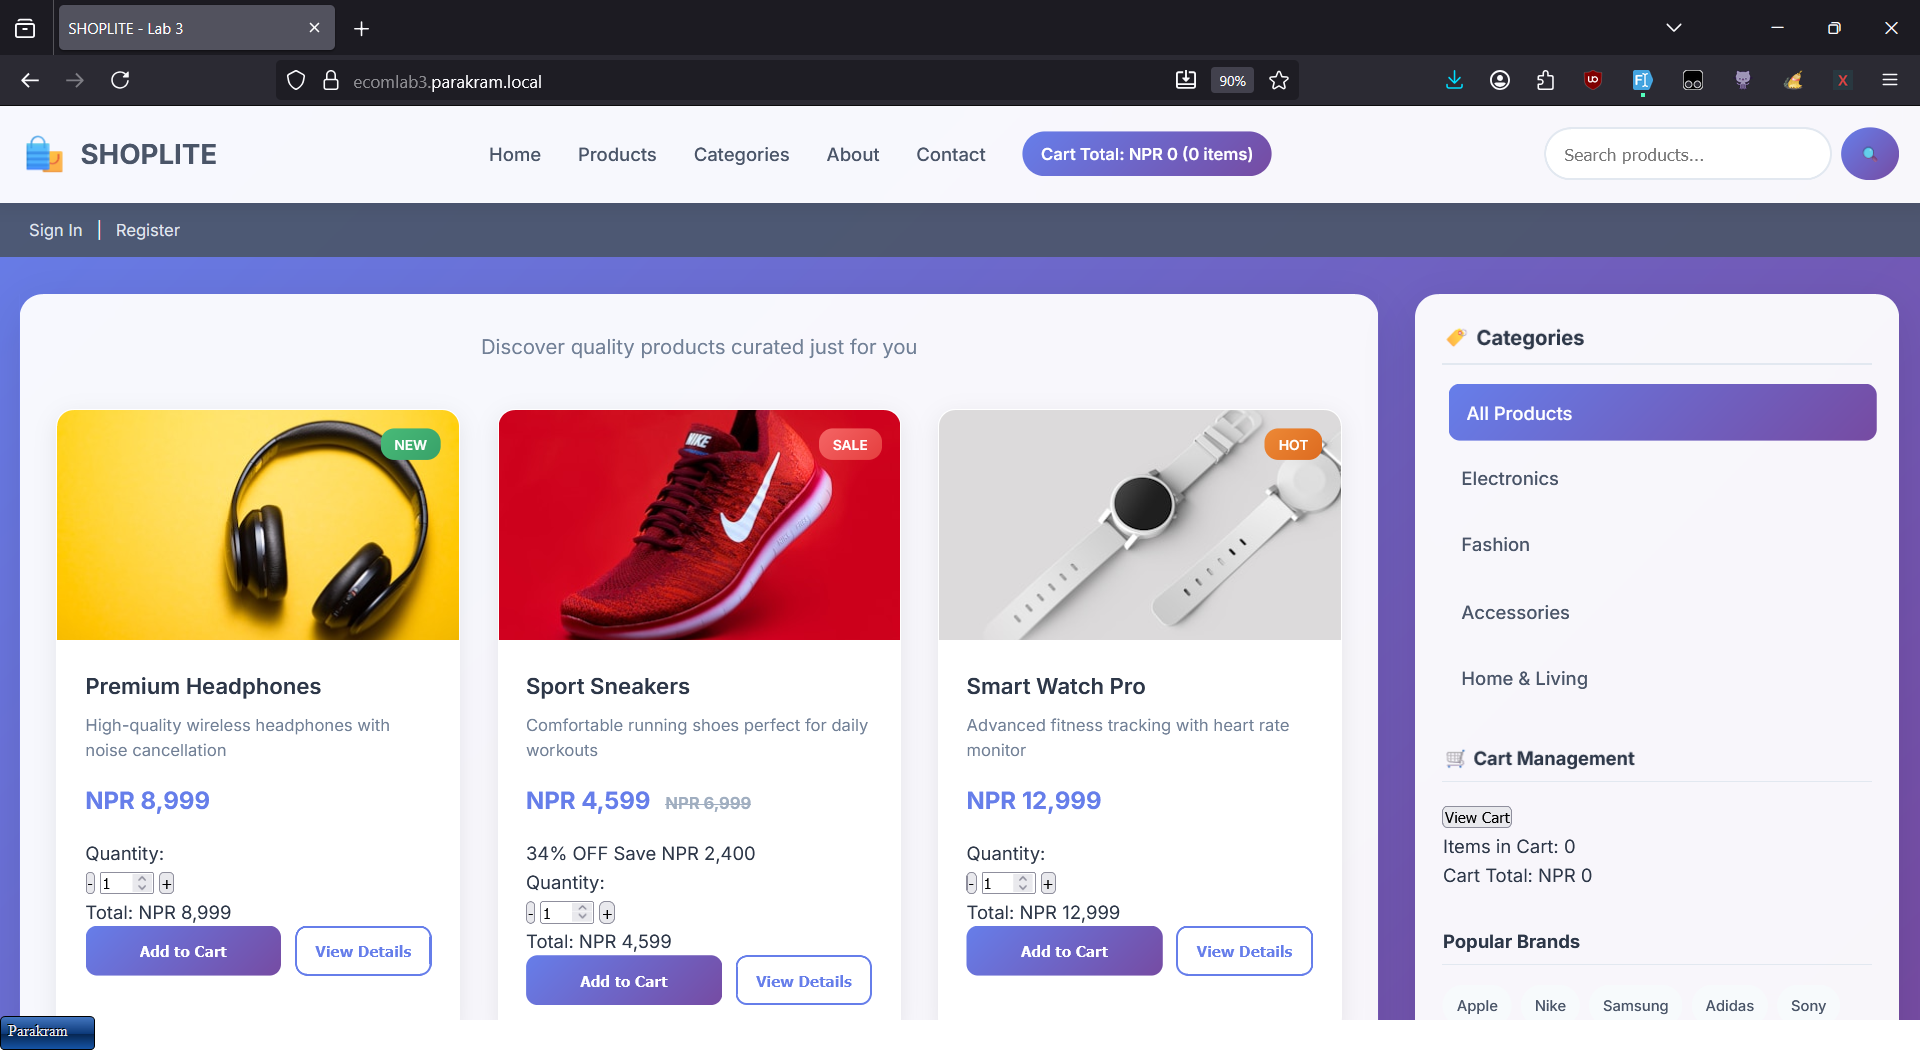
\includegraphics[width=\textwidth,height=6cm,keepaspectratio]{images/output1.png}
  \caption{Product Catalog.}
  \label{fig:img1}
\end{figure}

\begin{figure}[H]
  \centering
  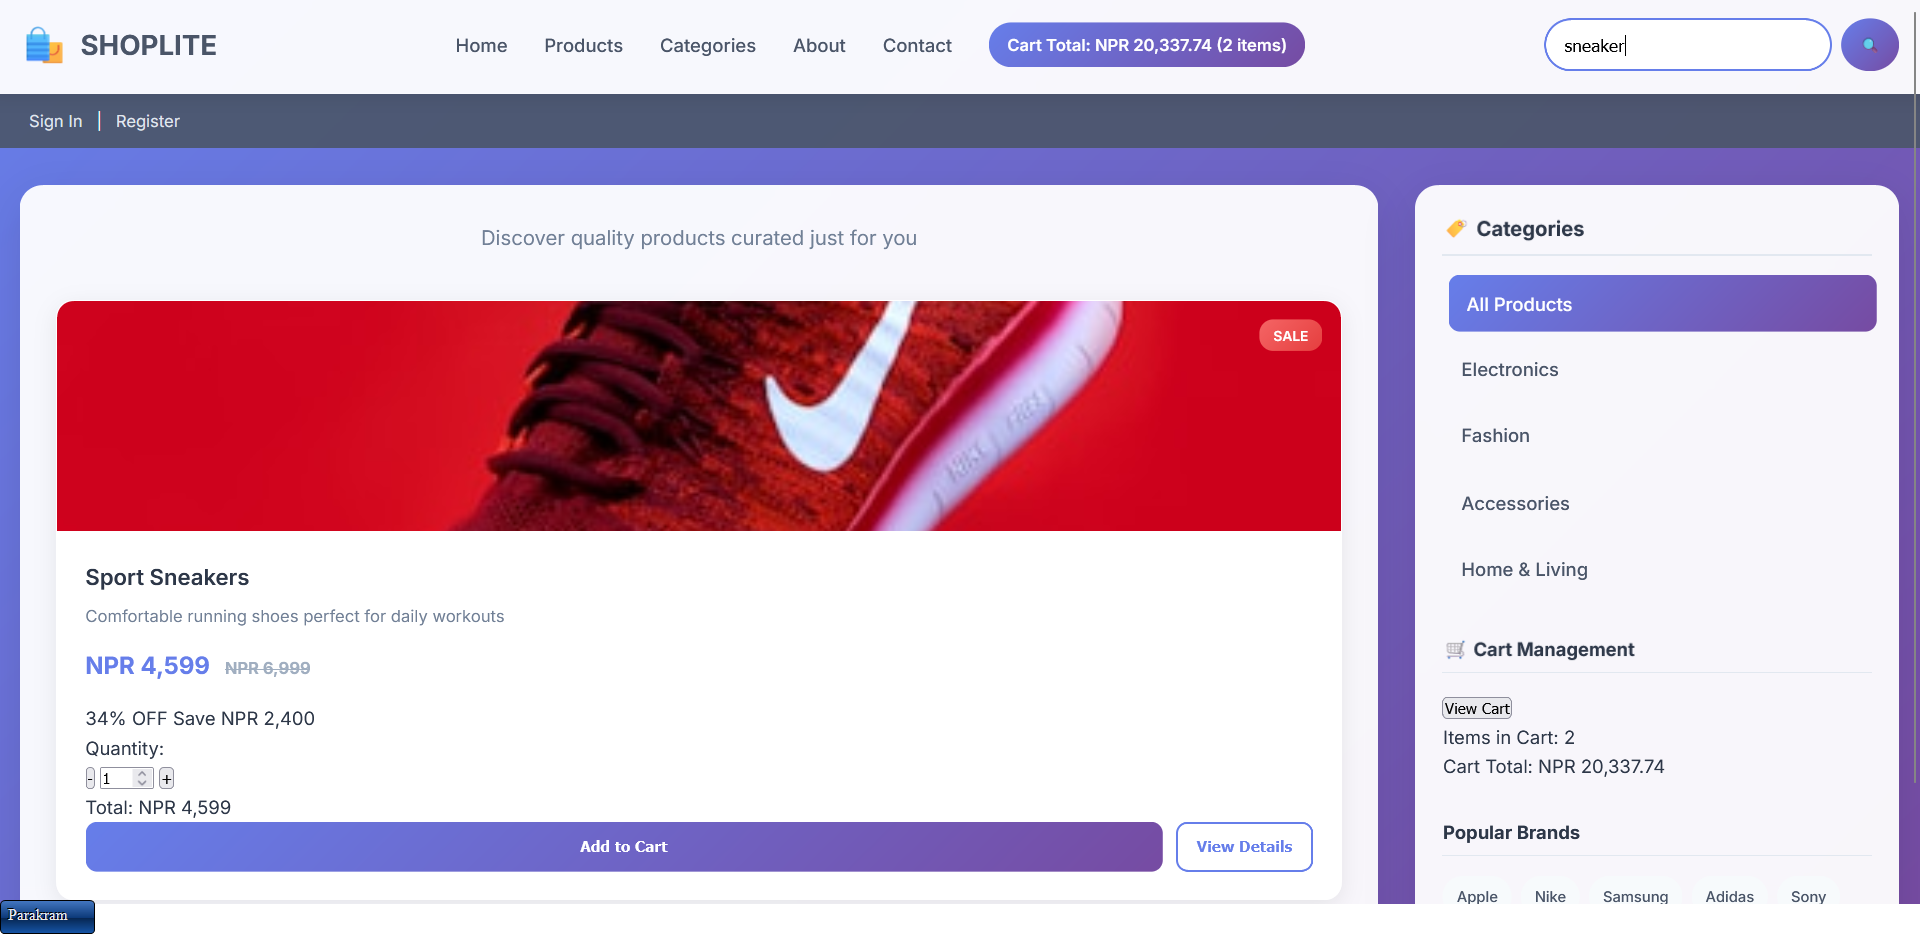
\includegraphics[width=0.7\textwidth,height=5cm,keepaspectratio]{images/output2.png}
  \caption{Product Search.}
  \label{fig:img2}
\end{figure}

\begin{figure}[H]
  \centering
  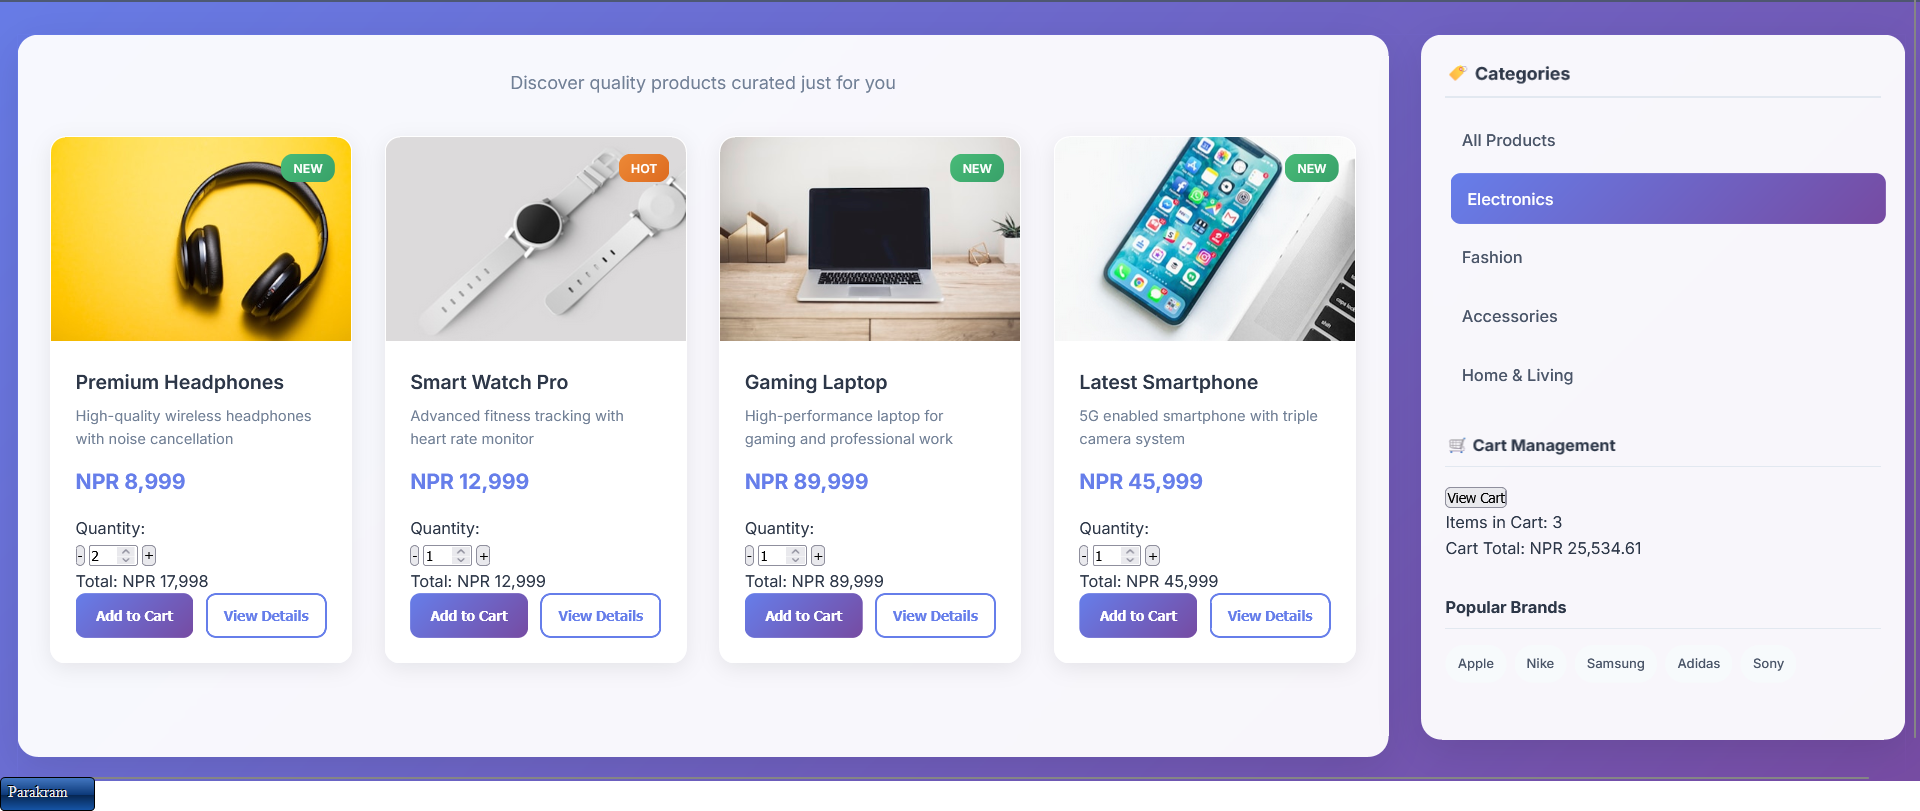
\includegraphics[width=\textwidth,height=6cm,keepaspectratio]{images/output3.png}
  \caption{Electronics Category.}
  \label{fig:img3}
\end{figure}

\begin{figure}[H]
  \centering
  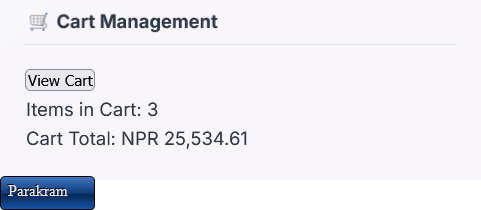
\includegraphics[width=\textwidth,height=6cm,keepaspectratio]{images/output4.png}
  \caption{Cart Info in Sidebar.}
  \label{fig:img4}
\end{figure}

\begin{figure}[H]
  \centering
  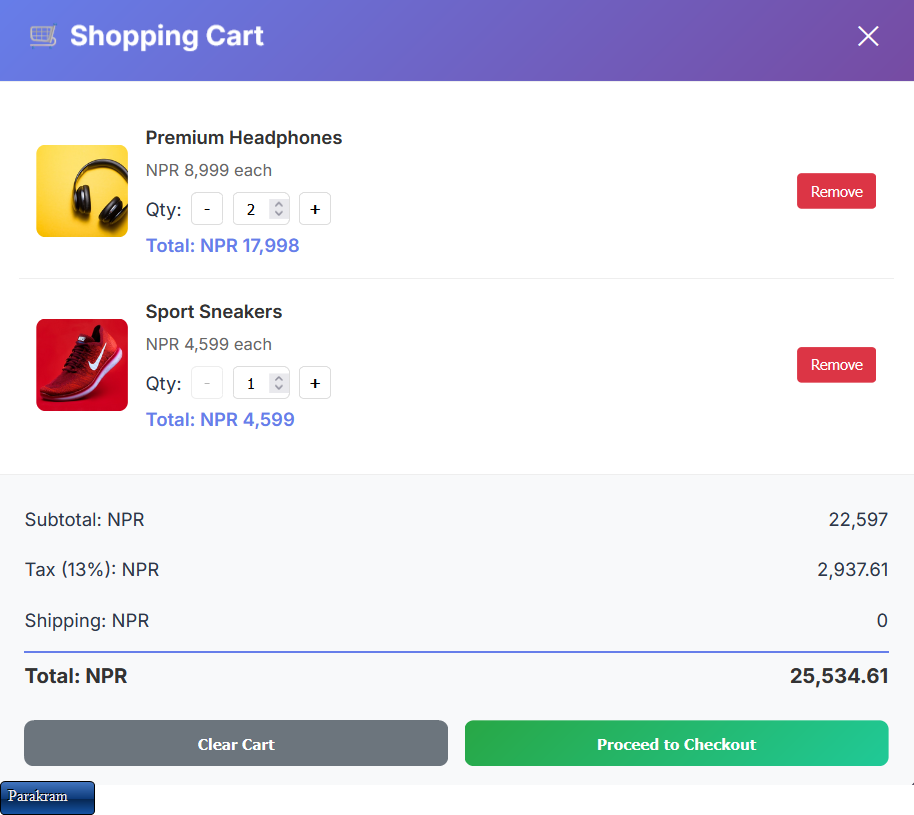
\includegraphics[width=\textwidth,height=6cm,keepaspectratio]{images/output5.png}
  \caption{View Cart.}
  \label{fig:img5}
\end{figure}

\begin{figure}[H]
  \centering
  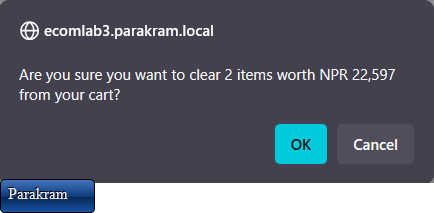
\includegraphics[width=\textwidth,height=6cm,keepaspectratio]{images/output6.png}
  \caption{Clear Cart Confirmation.}
  \label{fig:img6}
\end{figure}

\begin{figure}[H]
  \centering
  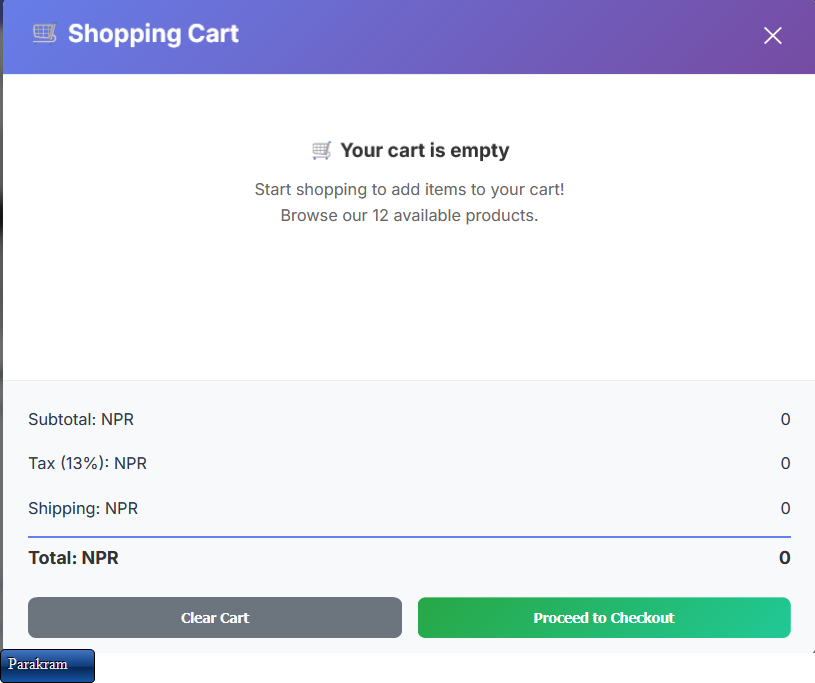
\includegraphics[width=\textwidth,height=6cm,keepaspectratio]{images/output7.png}
  \caption{Empty Cart.}
  \label{fig:img7}
\end{figure}

\section*{7. Result}
The e-commerce application successfully implemented comprehensive cart management using JavaScript arrays and objects. Features include dynamic cart operations with real-time item addition, modification, and removal using array methods like push(), splice(), and reduce(). The cart overlay displays items with persistent localStorage storage, automatic total calculations including tax and shipping, and complete DOM manipulation for seamless user interactions across all devices.

\section*{8. Conclusion}
This lab demonstrated advanced JavaScript programming concepts through practical e-commerce cart implementation. Students mastered array and object manipulation, learned essential array methods for data operations, and implemented sophisticated DOM manipulation techniques. The project established strong foundations in data structures, event-driven programming, and modern web storage, transforming static product displays into fully functional shopping cart systems with professional-grade user experience.

\section*{9. References}
\begin{itemize}
  \item \href{https://developer.mozilla.org/en-US/docs/Web/JavaScript/Reference/Global_Objects/Array}{MDN Array Methods Documentation}
  \item \href{https://developer.mozilla.org/en-US/docs/Web/API/Document_Object_Model}{MDN DOM Manipulation Guide}
  \item \href{https://developer.mozilla.org/en-US/docs/Web/API/Storage}{MDN Web Storage API}
  \item \href{https://javascript.info/array-methods}{Modern JavaScript Array Methods Tutorial}
\end{itemize}

\end{document}
